\documentclass[11pt]{scrartcl}
\usepackage[T1]{fontenc}
\usepackage[a4paper, left=3cm, right=2cm, top=2cm, bottom=2cm]{geometry}
\usepackage[activate]{pdfcprot}
\usepackage[ngerman]{babel}
\usepackage[parfill]{parskip}
\usepackage[utf8]{inputenc}
\usepackage{kurier}
\usepackage{amsmath}
\usepackage{amssymb}
\usepackage{xcolor}
\usepackage{epstopdf}
\usepackage{txfonts}
\usepackage{fancyhdr}
\usepackage{graphicx}
\usepackage{prettyref}
\usepackage{hyperref}
\usepackage{eurosym}
\usepackage{setspace}
\usepackage{units}
\usepackage{eso-pic,graphicx}
\usepackage{icomma}

\definecolor{darkblue}{rgb}{0,0,.5}
\hypersetup{pdftex=true, colorlinks=true, breaklinks=false, linkcolor=black, menucolor=black, pagecolor=black, urlcolor=darkblue}



\setlength{\columnsep}{2cm}


\newcommand{\arcsinh}{\mathrm{arcsinh}}
\newcommand{\asinh}{\mathrm{arcsinh}}
\newcommand{\ergebnis}{\textcolor{red}{\mathrm{Ergebnis}}}
\newcommand{\fehlt}{\textcolor{red}{Hier fehlen noch Inhalte.}}
\newcommand{\betanotice}{\textcolor{red}{Diese Aufgaben sind noch nicht in der Übung kontrolliert worden. Es sind lediglich meine Überlegungen und Lösungsansätze zu den Aufgaben. Es können Fehler enthalten sein!!! Das Dokument wird fortwährend aktualisiert und erst wenn das \textcolor{black}{beta} aus dem Dateinamen verschwindet ist es endgültig.}}
\newcommand{\half}{\frac{1}{2}}
\renewcommand{\d}{\, \mathrm d}
\newcommand{\punkte}{\textcolor{white}{xxxxx}}
\newcommand{\p}{\, \partial}
\newcommand{\dd}[1]{\item[#1] \hfill \\}

\renewcommand{\familydefault}{\sfdefault}



\newcommand{\themodul}{Probeklausuren 10+11}
\newcommand{\thetutor}{bei Prof. Schöning}

\pagestyle{fancy}
\fancyhead[L]{\footnotesize{C. Hansen}}
\chead{\thepage}
\rhead{}
\lfoot{}
\cfoot{}
\rfoot{}

\title{\themodul{}}
\publishers{\thetutor}


\author{Christoph Hansen \\ {\small \href{mailto:chris@university-material.de}{chris@university-material.de}} }

\date{}

\usepackage{paralist}
\begin{document}

\maketitle

Dieser Text ist unter der
\href{http://creativecommons.org/licenses/by-nc/4.0/}{Creative Commons CC BY-NC 4.0}
Lizenz veröffentlicht.

\textcolor{red}{%
    Ich erhebe keinen Anspruch auf Vollständigkeit oder Richtigkeit. Falls ihr
    Fehler findet oder etwas fehlt, dann meldet euch bitte über den
    Emailkontakt.
}


\tableofcontents

\newpage


\section{Klausur 10}

\subsection{Aufgabe 1}

Bei dieser Aufgabe bin ich mir nicht sicher, ob die jeweiligen Lösungen korrekt sind. Wenn jemand begründet eine bessere hat, dann soll er sich melden.

\hfill\\

\begin{center}
\begin{tabular}{c|c|c|c|c|c|c|c|c|c}
a) & b) & c) & d) & e) & f) & g) & h) & i) & j) \\ 
\hline 
R & R & R & F & F & R & R & R & R & F \\ 
\end{tabular} 
\end{center}


\subsection{Aufgabe 2}

\subsubsection*{a)}

mechanisch, thermisch, optisch, akustisch

\subsubsection*{b)}

\begin{figure}[h]
\centering
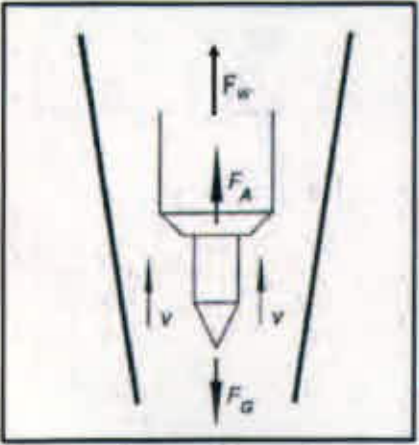
\includegraphics[scale=0.6]{A2b.png}
\caption{$F_A$: Auftriebskraft, $F_W$: Widerstandskraft, $F_G$: Gewichtskraft}
\end{figure}

Der zu messende Luftstrom wird von unten in die Apparatur eingeleitet und drückt den Schwebekörper nach oben. Nachdem sich der Schwebekörper auf eine konstante Höhe eingependelt hat, kann man die Durchflussmenge anhand der Höhe bestimmen.

\subsubsection*{c)}

\begin{align*}
\dot{V} &= \frac{1}{\sqrt{c_w}} \cdot \left( A_R - A_S \right) \cdot \sqrt{\frac{2 \cdot g \cdot V_s \cdot \left( \rho_s - \rho_m \right)}{\rho_m \cdot A_s}}
\end{align*}


\subsubsection*{d)}


\begin{align*}
\text{Gase:} \qquad &\unit[1]{l/h} - \unit[2000]{m^3/h} \\
\text{Flüssigkeiten:} \qquad &\unit[100]{ml/h} - \unit[100]{m^3/h} \\
\end{align*}

\subsubsection*{e)}

\begin{itemize}
\item Ultraschall Laufzeitverfahren
\item Ultraschall Doppler Verfahren
\item ??
\end{itemize}


\subsubsection*{f)}

\begin{figure}[h]
\centering
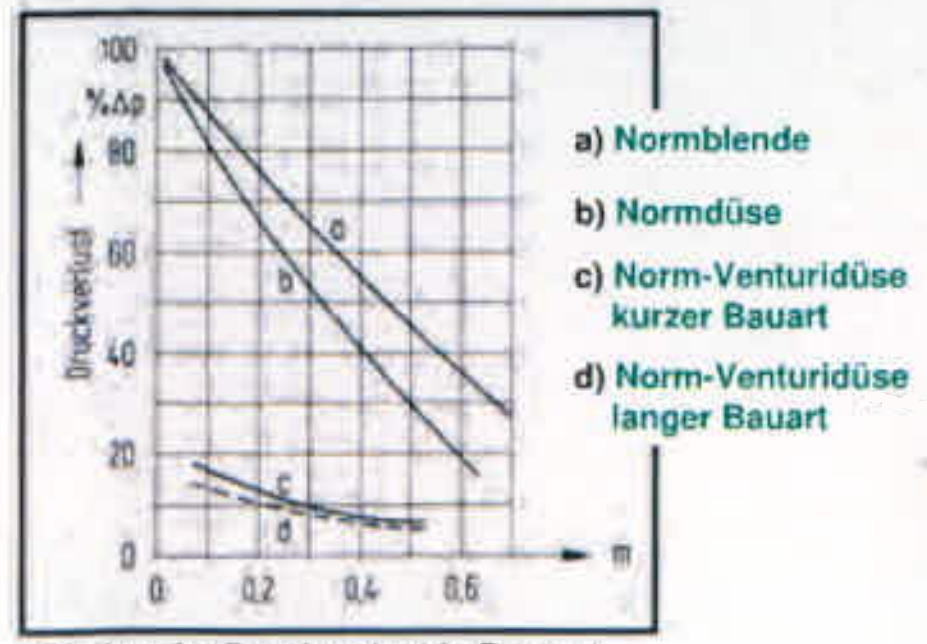
\includegraphics[scale=0.5]{A2f.png}
\end{figure}


\subsection{Aufgabe 3}

\subsubsection*{a)}

\[ R(\nu) = R_0 \cdot \left( 1 + \alpha \nu \right) \]

$R_0$: Widerstand bei $\unit[0]{^\circ C}$ \\
$\alpha$: Temperaturkoeffizient


\subsubsection*{b)}

\begin{align*}
U(60) &= 100 \cdot \left( 1 + 3,85 \cdot 10^{-3} \cdot 60 \right) \cdot 0,001 = \unit[123,1]{mV} \\
U(100) &= 100 \cdot \left( 1 + 3,85 \cdot 10^{-3} \cdot 100 \right) \cdot 0,001 = \unit[138,5]{mV}
\end{align*}


\subsubsection*{c)}

DIN A, bei DIN B ist die Abweichung bereits zu groß.


\subsubsection*{d)}

Wir berechnen zunächst die Genauigkeit bei $\unit[60]{^\circ C}$:

\begin{align*}
\Delta \nu &= 0,15 + 0,002 \cdot 60 = \unit[0,27]{^\circ C}
\intertext{Die Gleichung für den Widerstand müssen wir nun differenzieren:}
\frac{\p R}{\p \nu} &= R_0 \cdot \alpha
\intertext{Zusammen mit der Temperaturabweichung können wir nun die Widerstandsabweichung bestimmen:}
\Delta R &= R_0 \cdot \alpha \cdot \nu = 100 \cdot 3,85 \cdot 10^{-3} \cdot 0,27 = \unit[0,104]{\Omega}
\end{align*}

Bei $\unit[60]{^\circ C}$ darf der Widerstand als in den Grenzen von $\unit[123 \pm 0,104]{\Omega}$ schwanken.


\subsubsection*{e)}

Da wir mit Vierleitermesstechnik messen, spielen die Widerstände der Leitungen keine Rolle! Man misst also die berechneten $\unit[123,1]{mV}$.


\subsubsection*{f)}

\begin{align*}
P &= R \cdot I^2 = 123,1 \cdot 0,001^2 = \unit[1,23 \cdot 10^{-4}]{W} \\
\Rightarrow \Delta \nu &= 0,16 \cdot 0,123 = \unit[0,0196]{^\circ C} 
\end{align*}


\newpage

\subsection{Aufgabe 4}

\subsubsection*{a)}


Die Geschwindigkeit berechnen wir über $v = \frac{s}{t}$. Die Standardabweichung ist dann $\sigma = \sqrt{\frac{1}{n-1} \cdot \sum \left( v_i - \bar{v} \right)^2}$


\subsubsection*{b)}

Ich verstehe nicht wie Erwartungswerte aus einer Fehlerfortpflanzung berechnen soll!

\begin{align*}
s &= \unit[19,95 \pm 0,308]{m} \\
t &= \unit[9,59 \pm 0,06]{s} \\
v &= \unit[2,08 \pm 0,111]{m/s}
\end{align*}


\subsubsection*{c)}

keine Lösung vorhanden.


\begin{align*}
\bar{s} &= 19,95 \pm 0,13 \\
\bar{t} &= 9,59 \pm 4,28 \\
\bar{v} &= 2,08 \pm 0,04
\end{align*}



\section{Klausur 11}

\subsection{Aufgabe 1}

Bei dieser Aufgabe bin ich mir nicht sicher, ob die jeweiligen Lösungen korrekt sind. Wenn jemand begründet eine bessere hat, dann soll er sich melden.

\hfill\\

\begin{center}
\begin{tabular}{c|c|c|c|c|c|c|c|c|c}
a) & b) & c) & d) & e) & f) & g) & h) & i) & j) \\ 
\hline 
F & F & F & R & R & R & R & R & R & F \\ 
\end{tabular} 
\end{center}


\subsection{Aufgabe 2}

\subsubsection*{a)}

Eine Kennlinie gibt das Verhalten wieder, das ein Bauteil zeigt, wenn ich die Eingangsgröße variiere. Die Empfindlichkeit des Bauteil im jeweiligen Punkt wird dabei durch die Steigung der Kennlinie in diesem Punkt dargestellt. \\
Der Übertragungsfaktor ist einfach ein Proportionalitätsfaktor.


\subsubsection*{b)}

\begin{center}
    \begin{figure}[h]
        \begin{minipage}[hbt]{7cm}
            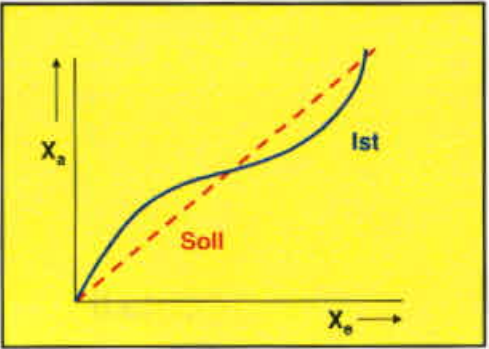
\includegraphics[width=6cm]{Kl112b_1.png}
            \caption{Linearitätsfehler}
        \end{minipage}
        %
        \begin{minipage}[hbt]{7cm}
            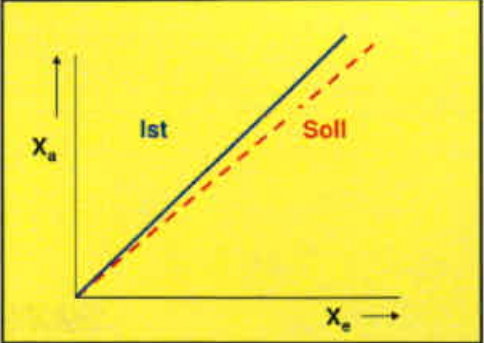
\includegraphics[width=6cm]{Kl112b_2.png}
            \caption{Übertragungsfaktorfehler}
        \end{minipage}
    \end{figure}
\end{center}

\begin{center}
    \begin{figure}[h]
        \begin{minipage}[hbt]{7cm}
            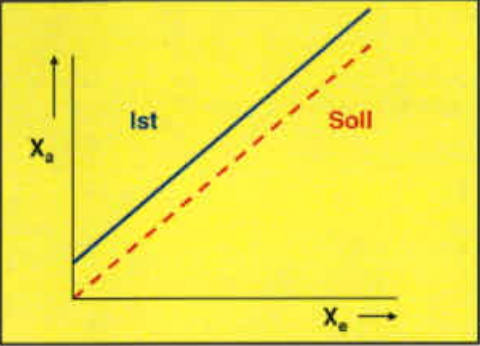
\includegraphics[width=6cm]{Kl112b_3.png}
            \caption{Offset}
        \end{minipage}
        %
        \begin{minipage}[hbt]{7cm}
            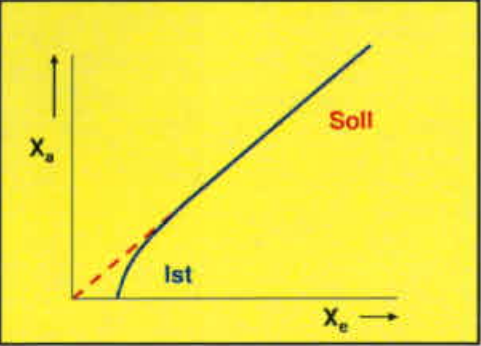
\includegraphics[width=6cm]{Kl112b_4.png}
            \caption{Ansprechunempfindlichkeit}
        \end{minipage}
    \end{figure}
\end{center}

\begin{center}
    \begin{figure}[h]
        \begin{minipage}[hbt]{7cm}
            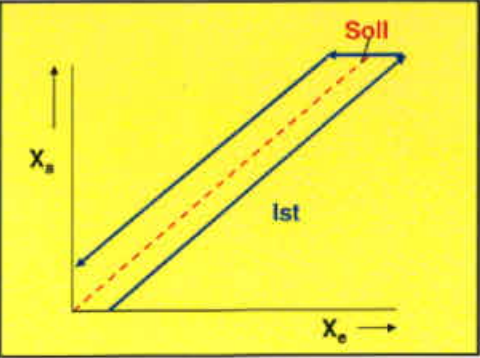
\includegraphics[width=6cm]{Kl112b_5.png}
            \caption{Hysterese}
        \end{minipage}
    \end{figure}
\end{center}


\subsection{Aufgabe 3}

\subsubsection*{a)}

\[ R(\nu) = R_0 \cdot \left( 1 + \alpha \nu \right) \]

$R_0$: Widerstand bei $\unit[0]{^\circ C}$ \\
$\alpha$: Temperaturkoeffizient


\subsubsection*{b)}

Die allgemeine Formel für den Widerstand ist:

\begin{align*}
R &= \frac{U}{I} = \frac{0,0958}{0,9978 \cdot 10^{-3}} = 96,01
\intertext{Für die Fehlerfortpflanzung müssen wir einmal nach der Spannung und einmal nach dem Strom ableiten:}
\frac{\p R}{\p U} &= \frac{1}{I} \\
\frac{\p R}{\p I} &= - \frac{U}{I^2}
\intertext{Nun setzen wir ein:}
\sigma &= \sqrt{\left( \frac{1}{I} \cdot S_U \right)^2 + \left( - \frac{U}{I^2} \cdot S_I \right)^2} \\ 
&= \sqrt{\left( \frac{1}{0,9978 \cdot 10^{-3}} \cdot 3,939 \cdot 10^{-4}  \right)^2 + \left( - \frac{0,0958}{\left(0,9978 \cdot 10^{-3} \right)^2} \cdot 5,8 \cdot 10^{-6} \right)^2} = \unit[0,68]{\Omega}
\intertext{Damit ist der Widerstand $\unit[96,01 \pm 0,68]{\Omega}$.}
\end{align*}


\subsubsection*{c)}

Ich rechne mit zunächst die Temperaturänderung eine PT-100 aus. Dazu nutzen wir die beiden Markanten Punkte von $\unit[100]{\Omega}$ bei $\unit[0]{^\circ C}$ und $\unit[120]{\Omega}$ bei $\unit[50]{^\circ C}$:

\begin{align*}
\frac{\unit[20]{\Omega}}{\unit[50]{K}} = \unit[0,4]{\Omega / K}
\intertext{Nun berechnen wir die Temperatur:}
96,01 &= 100 - 0,4 \cdot x \\
\Leftrightarrow x &= \unit[9,975]{K}
\end{align*}

Im Temperaturbereich um $\unit[-9,975]{^\circ C}$.


\subsubsection*{d)}

Der PT-100 ist ein passiver Sensor.


\subsubsection*{e)}

Die Schwingungen in konstanten Bereichen verschwinden.


\subsection{Aufgabe 4}

\subsubsection*{a)}

\begin{figure}[h]
\centering
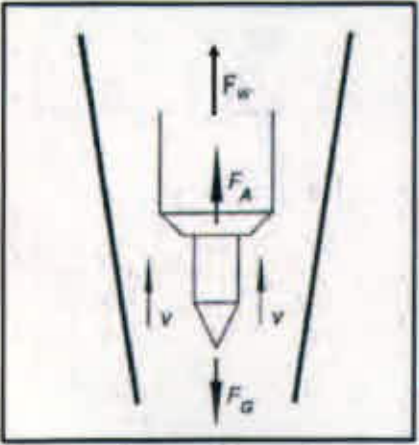
\includegraphics[scale=0.6]{A2b.png}
\caption{$F_A$: Auftriebskraft, $F_W$: Widerstandskraft, $F_G$: Gewichtskraft; $F_G = F_A + F_W$}
\end{figure}

Der zu messende Luftstrom wird von unten in die Apparatur eingeleitet und drückt den Schwebekörper nach oben. Nachdem sich der Schwebekörper auf eine konstante Höhe eingependelt hat, kann man die Durchflussmenge anhand der Höhe bestimmen.

\subsubsection*{c)}

\begin{align*}
\dot{V} &= \frac{1}{\sqrt{c_w}} \cdot \left( A_R - A_S \right) \cdot \sqrt{\frac{2 \cdot g \cdot V_s \cdot \left( \rho_s - \rho_m \right)}{\rho_m \cdot A_s}}
\end{align*}

\subsubsection*{d)}

Wir gehen nach dem gleichen Verfahren vor wie in der Übungsaufgabe 21. Wir definieren einen Volumenstrom $\dot{V_2'}$ der einer $100\%$ Anzeige entspricht und rechnen später zurück. Zuerst stellen wir die Ströme ins Verhältnis:

\begin{align*}
\frac{\dot{V_2'}}{\dot{V_1}} &= \frac{\frac{1}{\sqrt{c_W}} \cdot \left( A_R - A_S \right) \cdot \sqrt{\frac{2 \cdot g \cdot V_S \cdot \left( \rho_s - \rho_{m2} \right)}{A_S \cdot \rho_{m2}}}}{\frac{1}{\sqrt{c_W}} \cdot \left( A_R - A_S \right) \cdot \sqrt{\frac{2 \cdot g \cdot V_S \cdot \left( \rho_s - \rho_{m2} \right)}{A_S \cdot \rho_{m2}}}}
\intertext{Das fällt reduziert sich zu:}
&= \sqrt{\frac{\rho_{m1} \cdot \left( \rho_s - \rho_{m2} \right)}{\rho_{m2} \cdot \left( \rho_s - \rho_{m1} \right)}}
\intertext{Nun müssen wir die beiden Dichten in den beiden Zuständen berechnen:}
\rho_1 &= \frac{p_1}{R \cdot T_1} = \frac{101300}{287,14 \cdot 293,15} = \unit[1,203]{kg/m^3} \\
\rho_2 &= \frac{p_2}{R \cdot T_2} = \frac{200000}{287,14 \cdot 333,15} = \unit[2,091]{kg/m^3} \\
\intertext{Jetzt setzen wir in unsere Verhältnisgleichung ein:}
\frac{\dot{V_2'}}{\dot{V_1}} &= \sqrt{\frac{1,203 \cdot \left( 2700 - 2,091 \right)}{2,091 \cdot \left( 2700 - 1,203 \right)}} = 0,758
\intertext{Der richtige Volumenstrom berechnet sich dann so:}
\dot{V_2} &= 0,4 \cdot 0,758 \cdot 120 = \unit[36,4]{l/min}
\end{align*}






\end{document}
